\documentclass[a4paper,12pt]{article} % добавить leqno в [] для нумерации слева
\usepackage[a4paper,top=1.3cm,bottom=2cm,left=1.5cm,right=1.5cm,marginparwidth=0.75cm]{geometry}
%%% Работа с русским языком
\usepackage{cmap}					% поиск в PDF
\usepackage[warn]{mathtext} 		% русские буквы в фомулах
\usepackage[T2A]{fontenc}			% кодировка
\usepackage[utf8]{inputenc}			% кодировка исходного текста
\usepackage[english,russian]{babel}	% локализация и переносы
\usepackage{physics}
\usepackage{multirow}

%%% Нормальное размещение таблиц (писать [H] в окружении таблицы)
\usepackage{float}
\restylefloat{table}


\usepackage{graphicx}

\usepackage{wrapfig}
\usepackage{tabularx}

\usepackage{hyperref}
\usepackage[rgb]{xcolor}
\hypersetup{
	colorlinks=true,urlcolor=blue
}
\usepackage{pgfplots}
\pgfplotsset{compat=1.9}
%%% Дополнительная работа с математикой
\usepackage{amsmath,amsfonts,amssymb,amsthm,mathtools} % AMS
\usepackage{icomma} % "Умная" запятая: $0,2$ --- число, $0, 2$ --- перечисление

%% Номера формул
%\mathtoolsset{showonlyrefs=true} % Показывать номера только у тех формул, на которые есть \eqref{} в тексте.

%% Шрифты
\usepackage{euscript}	 % Шрифт Евклид
\usepackage{mathrsfs} % Красивый матшрифт

%% Свои команды
\DeclareMathOperator{\sgn}{\mathop{sgn}}

%% Перенос знаков в формулах (по Львовскому)
\newcommand*{\hm}[1]{#1\nobreak\discretionary{}
	{\hbox{$\mathsurround=0pt #1$}}{}}

\date{\today}

\begin{document}

\begin{titlepage}
	\begin{center}
		{\large МОСКОВСКИЙ ФИЗИКО-ТЕХНИЧЕСКИЙ ИНСТИТУТ (НАЦИОНАЛЬНЫЙ ИССЛЕДОВАТЕЛЬСКИЙ УНИВЕРСИТЕТ)}
	\end{center}
	\begin{center}
		{\large Физтех-школа физики и исследований им. Ландау}
	\end{center}
	
	
	\vspace{4.5cm}
	{\huge
		\begin{center}
			{\bf Отчёт о выполнении лабораторной работы №4.5.2}\\
			Интерференция лазерного излучения
		\end{center}
	}
	\vspace{2cm}
	\begin{flushright}
		{\LARGE Авторы:\\ Сенокосов Арсений Олегович \\ Сафин Дим Рустемович \\
			\vspace{0.2cm}
			Б02-012}
	\end{flushright}
	\vspace{8cm}
	\begin{center}
		Долгопрудный\\
		\today
	\end{center}
\end{titlepage}
%\numberwithin{equation}{section}

\section{Введение}

\textbf{Цель работы:} исследование видности интерференционной картины излучения гелий-неонового лазера и определение длины когерентности излучения.

\textbf{Оборудование:} He-Ne-лазер, интерферометр Майкельсона с подвижным зеркалом, фотодиод с усилителем, осциллограф, поляроид, линейка.

\section{Теоретическое введение}

Важный параметр интерференционной картины --- ее видность:

\begin{equation}\label{V0}
V = \dfrac{I_{max} - I_{min}}{I_{max} + I_{min}}
\end{equation}

Удобно представлять видимость в виде произведения функций различных параметров установки/системы:

\begin{equation}\label{VVV}
V = V_1 V_2 V_3
\end{equation}

Рассмотрим эти функции подробнее. Первая из них отвечает за отношение интенсивностей интерферирующих волн:

\begin{equation}\label{V1}
V_1 = \dfrac{2\sqrt{\delta}}{1 + \delta}, \quad \delta = \dfrac{B_m^2}{A_m^2}
\end{equation}


Здесь $ A_m, B_m $ --- амплитуды волн. Вторая функция учитывает влияние разности хода и спектрального состава волн:


\begin{equation}\label{}
\gamma_2 = \dfrac{\sum\limits_n A_n^2 \cos{\dfrac{2\pi \Delta \nu n l}{c}}}{\sum\limits_n A_n^2} \sim e^{-(\pi \Delta F l /c^2)}
\end{equation}

\begin{wrapfigure}{l}{0.35\linewidth} 
	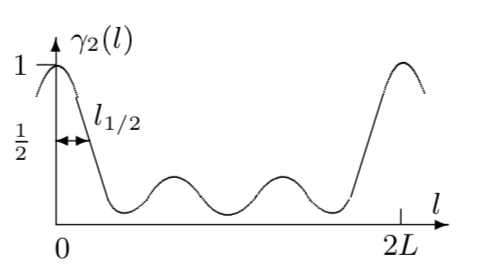
\includegraphics[width=\linewidth]{v2.png}
	\caption{Качественный график $ V_2 $}
	\label{V2graf}
\end{wrapfigure}


Здесь $ l $ --- разность хода, $ \Delta\nu $ --- спектральный состав излучения, $ A_n^2 $ --- интенсивность мод. Оценка приведена из перехода к непрерывному пределу. На графике (рис.\ref{V2graf}) показан вид $ V_2(l) $, позволяющий получить расстояние $ L $ между зеркалами резонатора и межмодовое расстояние $ \Delta \nu $. Величина $ l_{1/2} $  позволяет оценить диапазон частот $ \Delta F $.
Формулы связи межмодового расстояния и длины $ L $, а также $ l_{1/2} \; \text{и} \; \Delta F $ таковы:

\begin{equation}\label{dnu}
\Delta \nu = \dfrac{c}{2L}, \quad l_{1/2} \approx \dfrac{0,26 c}{\Delta F}
\end{equation}

Последняя функция --- зависимость от угла поляризации $ \alpha $:

\begin{equation}\label{}
V_3 = |\cos{\alpha}|
\end{equation}

\section{Экспериментальная установка}

\subsection{Описание установки}

Для получения интерференционной картины используется интерферометр Майкельсона, смонтированный на вертикально стоящей массивной металлической плите. Схема установки приведена на рисунке.

\begin{figure}[h!]
	\centering
	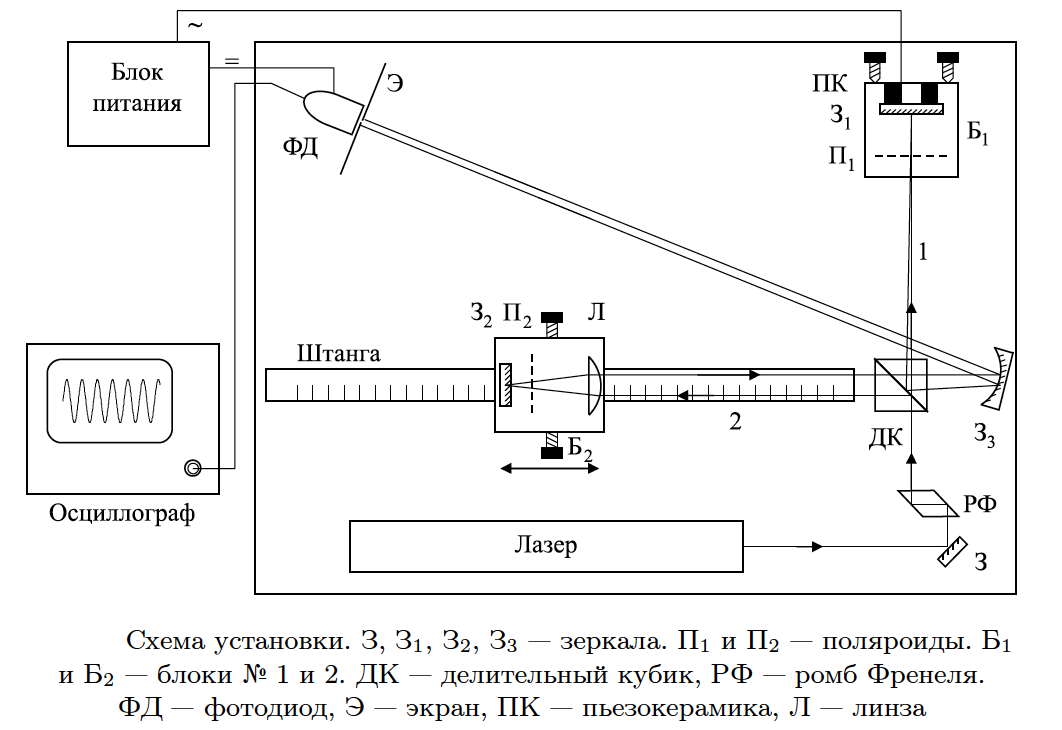
\includegraphics[width=\linewidth]{lab.png}
	%		\caption{Экспериментальная установка}
	\label{lab}
\end{figure}

Источником света служит гелий-неоновый лазер (средняя длина
волны $ \lambda_0 = 632,8 $ нм). Пучок лазерного излучения отражается от зеркала З и проходит призму полного внутреннего отражения РФ (ромб Френеля), которая превращает линейную поляризацию излучения в круговую. Если в установке используется лазер, излучающий неполяризованный свет, то ромб Френеля не нужен, но он и не мешает выполнению
работы. Далее лазерное излучение делится диагональной плоскостью
делительного кубика ДК на два пучка.

Пучок 1 проходит поляроид $ \text{П}_1, $ отражается под небольшим углом от зеркала $ \text{З}_1 $, снова проходит поляроид $ \text{П}_1 $ и, частично отражаясь от диагональной плоскости делительного кубика, выходит из интерферометра, попадает на зеркало $ \text{З}_3 $ и далее на фотодиод ФД. Зеркало $ \text{З}_1 $ наклеено на пьезокерамику ПК, которая может осуществлять малые колебания зеркала вдоль направления распространения падающего пучка. Поляроид и зеркало с пьезокерамикой собраны в единый блок $ \text{Б}_1 $, который крепится к вертикально стоящей плите. В блоке $ \text{Б}_1 $ имеются юстировочные винты, которые позволяют регулировать угол наклона зеркала $ \text{З}_1 $. В установке предусмотрена возможность вращения поляроида $ \text{П}_1 $. Угол поворота отсчитывается по шкале, нанесённой на оправу поляроида.
Пучок 2 проходит линзу Л, поляроид $ \text{П}_2 $, отражается от зеркала $ \text{З}_2 $, снова проходит поляроид $ \text{П}_2 $, линзу Л и делительный кубик, выходит из интерферометра, попадает на зеркало $ \text{З}_3 $ и далее на фотодиод ФД. Таким образом, от зеркала $ \text{З}_3 $ под небольшим углом друг к другу идут на фотодиод два пучка, прошедшие разные плечи интерферометра. Между ними происходит интерференция и образуются интерференционные полосы. Линза Л, поляроид $ \text{П}_2 $ и зеркало $ \text{З}_2 $ собраны в единый блок $ \text{Б}_2 $.

Зеркало $ \text{З}_2 $ установлено в фокальной плоскости линзы Л. Это сделано
для того, чтобы падающий и выходящий из блока $ \text{Б}_2 $ пучки всегда были
параллельны друг другу. Блок $ \text{Б}_2 $ может перемещаться вдоль пучка 2
по штанге, жёстко связанной с плитой интерферометра. Длина штанги
90 см. В установке предусмотрена возможность небольшого поперечно-
го перемещения блока $ \text{Б}_2 $, что позволяет регулировать расстояние меж-
ду падающим и выходящим из блока пучками. При измерениях блок
Б2 крепится к штанге при помощи двух винтов. Вдоль штанги нанесены деления через один сантиметр. При перемещении блока $ \text{Б}_2 $ вдоль
штанги на величину $ x_1 $ геометрическая разность хода между пучками
1 и 2 изменяется на величину $ l = 2x_1 $.

Сферическое зеркало $ \text{З}_3 $ с небольшим фокусным расстоянием увеличивает картину интерференционных полос и позволяет наблюдать её
на экране Э, расположенном в плоскости входного окна фотодиода.
Свет попадает на фотодиод ФД через узкую щель в центре экрана.
Щель ориентируется параллельно интерференционным полосам. Ширина щели меньше расстояния между полосами. Сигнал фотодиода усиливается и подаётся на вход осциллографа. Для питания усилителя
сигнала фотодиода и управления пьезокерамикой используется блок
питания БП.

На пьезокерамику подаётся напряжение с частотой 50 Гц. При этом
её длина изменяется с частотой 100 Гц. Величина удлинения зависит от
приложенного напряжения и регулируется ручкой "<Качание"> на блоке
питания. Обычно удлинение составляет несколько длин волн света. На
эту величину перемещается вдоль пучка 1 зеркало $ \text{З}_1 $. Интерференционная картина смещается на ширину полосы (одно колебание на экране осциллографа), если зеркало $ \text{З}_1 $ смещается на $ \lambda_0 /2 \sim 0,3 $ мкм. При
измерениях через входную щель фотодиода последовательно проходит
несколько полос интерференционной картины, а на экране осциллографа наблюдаются колебания с изменяющимся периодом.

\subsection{Методика измерения}

\begin{wrapfigure}{l}{0.35\linewidth} 
	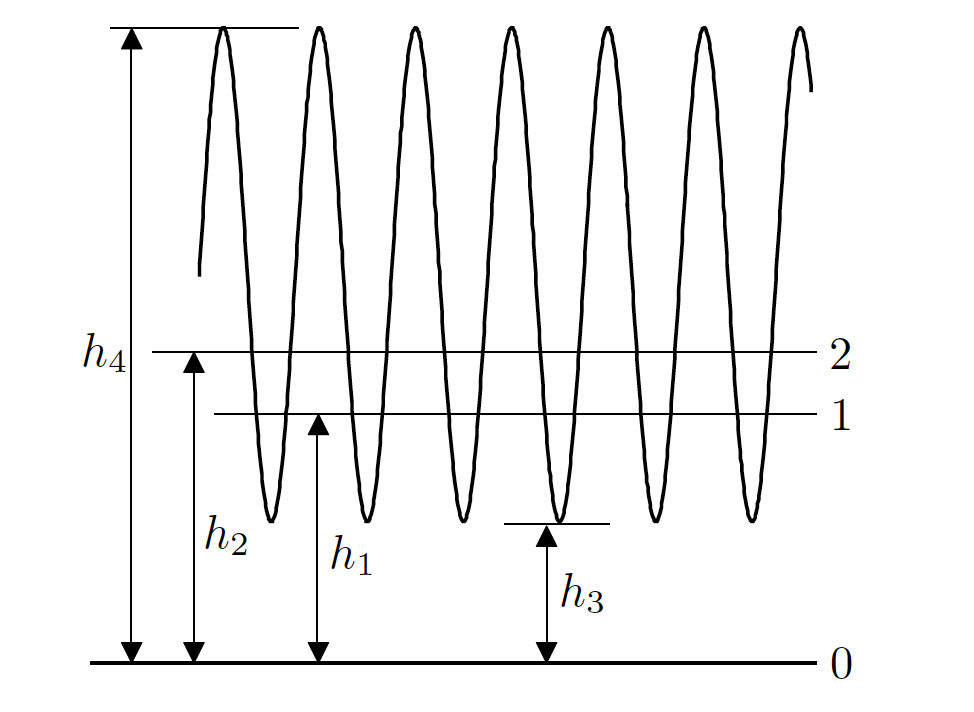
\includegraphics[width=\linewidth]{os}
	\caption{Сигнал фотодиода на осциллографе}
	\label{}
\end{wrapfigure}

Осциллограф мы используем для нахождения следующих вели-
чин: фоновой засветки (линия 0 --- перекрыты оба пучка 1 и 2); интенсивность света каждого из пучков (линии 1 или 2 --- перекрыт пучок
2 или 1); максимума и минимума интенсивности интерференционной
картины (открыты оба пучка). При этом параметр $ \delta $ из \eqref{V1},  определяется отношением

\begin{equation}\label{delta}
\delta = \dfrac{h_1}{h_2}
\end{equation}

Понятно, что из физического смысла, наша видимость рассчитывается очевидным образом, согласно формуле \eqref{V0}, так:

\begin{equation}\label{V}
V = \dfrac{h_4 - h_3}{h_4 + h_3}
\end{equation}

Отсюда, используя \eqref{VVV}, мы можем получить наши функции из \eqref{V}, фиксируя одну из них (т.е. беря равной единице). Так, при $ \alpha = 0 \Rightarrow V_3 = 1 $, 

\begin{equation}\label{V2}
V_2 (l) = \dfrac{V}{V_1} = \dfrac{h_4 - h_3}{h_4 + h_3} \cdot \dfrac{h_2}{h_1}
\end{equation}

А приняв разность хода $ l = 0 \Rightarrow V_2 = 0 $, можно найти 

\begin{equation}\label{V_3}
V_3(\alpha) = \dfrac{V}{V_1} = \dfrac{h_4 - h_3}{h_4 + h_3} \cdot \dfrac{h_2}{h_1}
\end{equation}


\section{Ход работы}


\subsection{Изучение поляризации}

Поворотами поляризатора $ \text{П}_1 $ убедимся, что свет от лазера --- поляризованный. Настроив поляроид на минимальную видимость и введя дополнительный поляроид, мы вновь получаем интерференционную картину при его поворотах. Интенсивность излучения при вращении поляроида меняется, что говорит о его \textbf{не хаотической} поляризации. При вращении также изменяется интерференционная картина, что говорит о \textbf{линейной или круговой} поляризации, а не хаотической.

\begin{table}[H]
	\caption{Измерение зависимости видности от угла}
	\begin{center}
		\begin{tabular}{|c|c|c|c|c|c|c|c|c|}
			\hline
			$ 	\alpha  $ & $ h_4 $ &  $ h_3 $& $ h_2 $ & $ h_1 $ & $ V $ & $  \delta  $ & $ V_1 $ & $ V_3 $ \\
			\hline
			5   & 32 & 25 & 16 & 13 & 0.12 & 0.81 & 0.99 & 0.12 \\
			15  & 33 & 23 & 16 & 12 & 0.18 & 0.75 & 0.99 & 0.18 \\
			25  & 37 & 23 & 16 & 15 & 0.23 & 0.94 & 1.00 & 0.23 \\
			35  & 38 & 21 & 16 & 15 & 0.29 & 0.94 & 1.00 & 0.29 \\
			40  & 34 & 18 & 16 & 10 & 0.31 & 0.63 & 0.97 & 0.32 \\
			45  & 35 & 17 & 16 & 11 & 0.35 & 0.69 & 0.98 & 0.35 \\
			50  & 35 & 16 & 16 & 11 & 0.37 & 0.69 & 0.98 & 0.38 \\
			60  & 29 & 14 & 16 & 6  & 0.35 & 0.38 & 0.89 & 0.39 \\
			70  & 28 & 13 & 16 & 6  & 0.37 & 0.38 & 0.89 & 0.41 \\
			80  & 27 & 13 & 16 & 5  & 0.35 & 0.31 & 0.85 & 0.41 \\
			90  & 24 & 13 & 16 & 4  & 0.30 & 0.25 & 0.80 & 0.37 \\
			100 & 24 & 14 & 16 & 4  & 0.26 & 0.25 & 0.80 & 0.33 \\
			110 & 22 & 14 & 16 & 3  & 0.22 & 0.19 & 0.73 & 0.30 \\
			120 & 22 & 15 & 16 & 3  & 0.19 & 0.19 & 0.73 & 0.26 \\
			130 & 22 & 16 & 16 & 3  & 0.16 & 0.19 & 0.73 & 0.22 \\
			140 & 22 & 17 & 16 & 4  & 0.13 & 0.25 & 0.80 & 0.16 \\
			150 & 23 & 19 & 17 & 5  & 0.10 & 0.29 & 0.84 & 0.11 \\
			160 & 24 & 22 & 17 & 7  & 0.04 & 0.41 & 0.91 & 0.05 \\
			\hline
		\end{tabular}
	\end{center}
	\label{table_v3}
\end{table}

\subsection{Измерение зависимости видности от угла}

Исследуем зависимость видности интерференционной картины от угла
$ \alpha $ поворота поляроида $ \text{П}_1 $ при нулевой разности хода ($ V_2 = 1 $). Для этого измерим величины $ h_1, h_2, h_3 \; \text{и} \; h_4 $ на экране осциллографа. Результаты занесем в таблицу \ref{table_v3} и построим график согласно формуле \eqref{V_3}. Значения для $ \delta, V, V_1 $ получим из формул выше.


\begin{center}
	\begin{tikzpicture}
	\begin{axis}[
	title={График 1 \quad Измерение зависимости видности $ V_3 $ от угла поляризации $ \alpha $},
	xlabel={$ \alpha, \; ^\circ $},
	ylabel={$ V_3 $},
	legend pos=north east,
	xmajorgrids=true,
	ymajorgrids=true,
	grid style=dashed,
	width = 520,
	height = 230,
	%xmin = 300,
	%xmax = 335,
	%ymin =40,
	%ymax =0.22,
	]
	\legend{ 
		Результат измерений,
		Аппроксимация $ \sin^2\alpha $
	};
	\addplot+ [blue, only marks, mark size = 4pt,
	error bars/.cd,
	x dir=both, x explicit,
	y dir=both, y explicit, 
	] table [x = T, y = sigma] {
		T	sigma         
		5	0.123469452
		15	0.180421959
		25	0.233454829
		35	0.288285625
		40	0.316227766
		45	0.352246427
		50	0.379106176
		60	0.391633534
		70	0.410737609
		80	0.410877491
		90	0.371621622
		100	0.328947368
		110	0.304712642
		120	0.25941752
		130	0.216506351
		140	0.16025641
		150	0.11363024
		160	0.047827748
		
	};
	\addplot [red, domain=0:170, line width =3.2pt] {0.00789+0.39687*(sin((pi*(x+0.6416*180/pi)/(3.87765))))^2};
	\end{axis}
	\end{tikzpicture}
\end{center}


Из графика следует, что он приближается функцией $ \cos^2 \alpha $. Это значит, что \textbf{поляризация --- линейная}. Выполняется \textbf{закон Малюса}:
\[ I = I_0 \cos^2\alpha \]


\subsection{Измерение зависимости видности от дальности хода}

Теперь установим $ \alpha $ на максимальную видность и будем перемещать блок $ \text{Б}_2 $, тем самым изменяя дальность хода $ x $. Аналогично предыдущему пункту измерим величины $ h_1, h_2, h_3 \; \text{и} \; h_4 $ на экране осциллографа. Результаты занесем в таблицу \ref{table_v2} и построим график согласно формуле \eqref{V2}. Значения для $ \delta, V, V_1 $ получим из формул выше.

\begin{table}[h!]
	\caption{Измерение зависимости видности от разности хода}
	\begin{center}
		\begin{tabular}{|c|c|c|c|c|c|c|c|c|}
			\hline
			$ 	x  $ & $ h_4 $ &  $ h_3 $& $ h_2 $ & $ h_1 $ & $ V $ & $  \delta  $ & $ V_1 $ & $ V_2 $ \\
			\hline
			11 & 18 & 7  & 6  & 8  & 0.44 & 1.33 & 0.99 & 0.44 \\
			12 & 16 & 7  & 4  & 8  & 0.39 & 2.00 & 0.94 & 0.42 \\
			14 & 28 & 9  & 11 & 8  & 0.51 & 0.73 & 0.99 & 0.52 \\
			16 & 37 & 18 & 17 & 11 & 0.35 & 0.65 & 0.98 & 0.35 \\
			17 & 39 & 17 & 18 & 16 & 0.39 & 0.89 & 1.00 & 0.39 \\
			18 & 39 & 19 & 19 & 11 & 0.34 & 0.58 & 0.96 & 0.36 \\
			20 & 33 & 17 & 15 & 11 & 0.32 & 0.73 & 0.99 & 0.32 \\
			22 & 37 & 21 & 19 & 11 & 0.28 & 0.58 & 0.96 & 0.29 \\
			24 & 33 & 25 & 22 & 11 & 0.14 & 0.50 & 0.94 & 0.15 \\
			26 & 27 & 20 & 14 & 11 & 0.15 & 0.79 & 0.99 & 0.15 \\
			28 & 24 & 19 & 12 & 11 & 0.12 & 0.92 & 1.00 & 0.12 \\
			30 & 28 & 24 & 16 & 11 & 0.08 & 0.69 & 0.98 & 0.08 \\
			32 & 35 & 32 & 23 & 11 & 0.04 & 0.48 & 0.94 & 0.05 \\
			34 & 30 & 27 & 18 & 11 & 0.05 & 0.61 & 0.97 & 0.05 \\
			36 & 32 & 30 & 21 & 11 & 0.03 & 0.52 & 0.95 & 0.03 \\
			38 & 19 & 18 & 8  & 10 & 0.03 & 1.25 & 0.99 & 0.03 \\
			40 & 13 & 12 & 3  & 10 & 0.04 & 3.33 & 0.84 & 0.05 \\
			42 & 17 & 15 & 7  & 10 & 0.06 & 1.43 & 0.98 & 0.06 \\
			44 & 27 & 22 & 17 & 10 & 0.10 & 0.59 & 0.97 & 0.11 \\
			46 & 29 & 21 & 17 & 8  & 0.16 & 0.47 & 0.93 & 0.17 \\
			48 & 30 & 18 & 16 & 8  & 0.25 & 0.50 & 0.94 & 0.27 \\
			50 & 21 & 18 & 12 & 8  & 0.08 & 0.67 & 0.98 & 0.08 \\
			52 & 22 & 20 & 13 & 9  & 0.05 & 0.69 & 0.98 & 0.05 \\
			54 & 16 & 15 & 6  & 10 & 0.03 & 1.67 & 0.97 & 0.03 \\
			56 & 17 & 15 & 9  & 7  & 0.06 & 0.78 & 0.99 & 0.06 \\
			58 & 16 & 14 & 9  & 7  & 0.07 & 0.78 & 0.99 & 0.07 \\
			60 & 17 & 15 & 10 & 8  & 0.06 & 0.80 & 0.99 & 0.06 \\
			62 & 18 & 14 & 10 & 7  & 0.13 & 0.70 & 0.98 & 0.13 \\
			64 & 15 & 11 & 11 & 7  & 0.15 & 0.64 & 0.97 & 0.16 \\
			66 & 19 & 16 & 13 & 5  & 0.09 & 0.38 & 0.90 & 0.10 \\
			68 & 36 & 29 & 26 & 8  & 0.11 & 0.31 & 0.85 & 0.13 \\
			72 & 21 & 13 & 10 & 8  & 0.24 & 0.80 & 0.99 & 0.24 \\
			74 & 16 & 10 & 6  & 7  & 0.23 & 1.17 & 1.00 & 0.23 \\
			76 & 28 & 13 & 14 & 8  & 0.37 & 0.57 & 0.96 & 0.38 \\
			78 & 22 & 5  & 8  & 6  & 0.63 & 0.75 & 0.99 & 0.64 \\
			80 & 22 & 7  & 7  & 8  & 0.52 & 1.14 & 1.00 & 0.52 \\
			82 & 24 & 8  & 9  & 8  & 0.50 & 0.89 & 1.00 & 0.50 \\
			84 & 28 & 11 & 12 & 8  & 0.44 & 0.67 & 0.98 & 0.44 \\
			\hline
		\end{tabular}
	\end{center}
	\label{table_v2}
\end{table}

\begin{center}
	\begin{tikzpicture}
	\begin{axis}[
	title={График 2 \quad Измерение зависимости видности $ V_2 $ от разности хода $ x $},
	xlabel={$ x $, см},
	ylabel={$ V_2 $},
	legend pos=north west,
	xmajorgrids=true,
	ymajorgrids=true,
	grid style=dashed,
	width = 520,
	height = 350,
	%xmin = 300,
	%xmax = 335,
	%ymin =40,
	%ymax =0.22,
	]
	\legend{ 
		Результат измерений,
		Аппроксимация $ \sin^2\alpha $
	};
	\addplot+ [blue, only marks, mark size = 4pt,
	error bars/.cd,
	x dir=both, x explicit,
	y dir=both, y explicit, 
	] table [x = T, y = sigma] {
		T	sigma         
		11	0.444559707
		12	0.415040937
		14	0.520036882
		16	0.353669936
		17	0.393538595
		18	0.357783343
		20	0.323855561
		22	0.286226675
		24	0.146297955
		26	0.150020233
		28	0.11638913
		30	0.078276984
		32	0.047855859
		34	0.05423527
		36	0.033958797
		38	0.027195421
		40	0.047469288
		42	0.06349652
		44	0.10565334
		46	0.171498585
		48	0.265165043
		50	0.078509287
		52	0.048426208
		54	0.033315986
		56	0.062994079
		58	0.067193684
		60	0.062889412
		62	0.12699304
		64	0.157791567
		66	0.095683938
		68	0.126941006
		72	0.236760139
		74	0.231455025
		76	0.380269134
		78	0.636154463
		80	0.51839465
		82	0.500867303
		84	0.444885958
		
		
	};

	\end{axis}
	\end{tikzpicture}
\end{center}

Видно, что у нас наблюдается 2 максимума по краям области измерения и некоторые колебания в промежуточной области. А именно, максимумы в области $ x_1 \approx (14 \pm 2) \; \text{см} $ и в области $ x_2 \approx (78 \pm 2) \; \text{см} $, откуда получаем следующий результат:

\begin{equation}\label{}
L = \dfrac{1}{2} (x_2 - x_1) = (32,0 \pm 1,4) \; \text{см}
\end{equation}

Отсюда нетрудно получить и значение $ \Delta \nu $ из формулы \eqref{dnu}:

\begin{equation}\label{}
\Delta \nu = \dfrac{c}{2L} \approx (4,7 \pm 0,2) \cdot 10^8 \; \text{Гц}
\end{equation}

Оценим $ l_{1/2} \approx (22 - 14) \text{ см} = (8 \pm 2) \text{ см} $, откуда по формуле \eqref{dnu} получаем

\begin{equation}\label{}
2\Delta F = 2\cdot \dfrac{0,26 c}{l_{1/2}} \approx (19,5 \pm 4,9) \cdot 10^8 \; \text{Гц}
\end{equation}

Тогда для числа одновременно генерируемых лазером продольных волн можно провести оценку:

\begin{equation}\label{}
N \approx 1 + \dfrac{ 2\Delta F}{\Delta \nu} \approx 5 \pm 1
\end{equation}


\section{Вывод}
\begin{itemize}
    \item В ходе выполнения лабораторная работы была изучена поляризация излучения лазера. При этом было установлено, что при вращении поляроида интенсивность излучения меняется, что говорит о его не хаотической поляризации. При этом изменяется и интерференционная картина. По этим результатам можно предположить, что поляризация \textbf{линейная} или \textbf{круговая}.
    \item Затем была исследована зависимость видности интерференционной картины от угла поляроида $ \text{П}_1 $. Из результатов измерений и аппроксимации следует, что зависимость приближается функцией $ \cos^2 \alpha $. Это значит, что поляризация излучения --- \textbf{линейная} согласно закону Малюса.
    \item В заключительной части работы была исследована зависимости видности интерференционной картины от разности хода. По полученным данным было оценено расстояние между максимумами, расстояние $ L $ между зеркалами оптического резонатора лазера, а также межмодовое расстояние $ \Delta\nu $. Для этих величин были получены следующие результаты:
    \[ \boxed{L = (32,0 \pm 1,4) \text{ см}} \]
    \[ \boxed{\Delta\nu = (4,7 \pm 0,2) \cdot 10^8 \text{ Гц}} \]
    \item Также по графику также было оценена полуширина $ l_{1/2} $. При помощи этих данных было получен диапазон частот $ 2\Delta F $, в котором происходит генерация продольных мод, и приблизительное число мод. Были получены следующие результаты:
    \[ \boxed{l_{1/2} = (8 \pm 2) \text{ см}} \]
    \[ \boxed{2\Delta F = (19,5 \pm 4,9)\cdot 10^8 \text{ Гц}} \]
    \[ \boxed{N = 5 \pm 1} \]
    \item Основной вклад в погрешнсть в ходе выполнения работы могла внести ошибка при определении продольного сдвига второго зеркального блока. Также не всегда было реальным точное измерение максимумов напряжений по показаниям осциллографа в силу их изменения во времени.
\end{itemize}








\end{document}